\chapter{Introduction}
\label{ch:intro}
The target of this chapter is to set the context of this thesis by outlining the importance and implications of Customer Satisfaction with regard to the business point of view as well as providing an overview on the capabilities of customer knowledge data to analyze a customers behavior related to a software product. 

\section{Customer Satisfaction as Business Value}
While companies were only focused on the quality of their products and services until the 1980s, increasing supply and resulting competition on the market caused a shift towards a more customer centric approach starting in the early 1990s \cite{neckel2015}. The trend is visualized in figure~\ref{fig:introDevelopment}. 

\begin{figure}
	\centering
		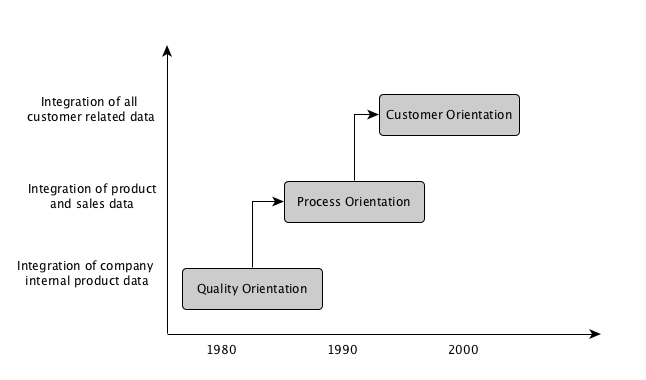
\includegraphics[width=1.0\textwidth]{img/introDevelopment.png}
	\caption{Development towards a customer centric company \cite{neckel2015}}
	\label{fig:introDevelopment}
\end{figure} 

Companies started to realize that the customer is an essential part of the company and has major influence on success and profitability. Furthermore, due to the oversupply of products and services, the competitive pressure has become higher over the last years . Especially online services and products have become extremely popular and people usually have a variety of similar ones to choose from. As a consequence this means that customers rarely stay at the same service provider due to convenience only since switching to a competitor has never been easier \cite{rygielski2002data}. For businesses it gets harder to attract and recruit new customers. As a result, keeping customers turns out to be a major business issue \cite{nerdinger2015}. As of \cite{chen2003understanding} the Boston Consulting Groups estimates that it costs 6.80\$ in the web world to care about existing customers and market them appropriately whereas acquiring a new web customer costs about 34\$. The described shift impacts the strategy how products are presented and marketed to the customer. To achieve the goal of successfully binding customers to the provided products and services, it is not sufficient anymore to pursue a traditional mass marketing strategy like sending the same advertising prospect to all the customers in a given area. This can even lead to a negative attitude of customers towards a company and to a potential break up of the relationship \cite{rygielski2002data, neckel2015}. Instead companies have to treat customers individually as they differ in their personality, behavior and needs. In a company which is centered around the customer, products have to be built to meet the customer needs \cite{chen2003understanding}. Apparently, no company can ever know each customer and his/her needs in depth at any point in time without collecting useful data about them. With the beginning of the 21st century a new hyped business term has been established, namely CRM (Customer Relationship Management). It can be described as the comprehensive process of knowing customers needs and wants, presenting the correct products and services via the preferred channels to them, allowing a convenient purchase of the selected product or service and providing good care after the purchase \cite{rygielski2002data}. CRM can be seen as the core process to establish profitable long-term relationships, develop customer loyalty and thus increase the value of the company. Although it has become widely recognized, different researchers look at it from various viewpoints and there is no unique valid definition. Some of them put their focus more on the processes and tools whereas others put more emphasis on the marketing aspect. All these different definitions available in literature have a common property of understanding the customer in detail \cite{Ngai2009}. However, the way of creating profitable customer relationships is hard and takes place on a fine line. It can be imagined as a pyramid where each level is based on the fundament below and removing one level can lead to destruction of the whole construct. The pyramid is visualized in figure~\ref{fig:introPyramid} and will be discussed in more detail. 

\begin{figure}
	\centering
	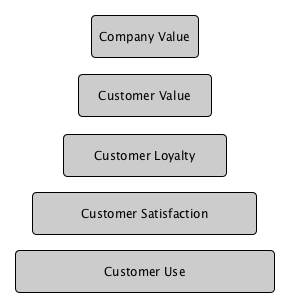
\includegraphics[width=0.5\textwidth]{img/introPyramid.png}
	\caption{Illustration of the way towards increasing company value \cite{neckel2015}}
	\label{fig:introPyramid}
\end{figure} 

\subsection{Customer Use}
With a seemingly unlimited number of marketing instruments and possibilities to influence people and drive them into a specific direction, it is often overseen that the basis for any customer relationship is the actual use of the product to solve an existing problem. If people do not see any sense of a product to solve a particular problem or make something easier in their lives, they will not buy it and any of higher levels on the pyramid will not work. Any successful product has its basis use case which solves a customers problem. However, in addition to this core use, products have to provide some extra value in order to communicate some unique value which makes the product standing out from the competitors. \cite{neckel2015}. In the service sector this can be summarized as service quality \cite{hussain2015service}. A good example for its customer use is definitely Apple Inc with their iPhone. In a simplified manner they manage to provide the base value of a current smartphone and since many years they are able to stand out of the competition with their unique and elegant design which gives customers a positive image and increases their reputation.

\subsection{Customer Satisfaction}
\label{ssec:customerSatisfaction}
The key topic this thesis cares about, is one of the major pillars in the CRM construct as illustrated in figure \ref{fig:introPyramid}. It was found out that Customer Satisfaction has a positive effect on the company value in the long-term. Costs for customer support drop, customers extend their relationship which has significant impact on overall costs. However, reasoning about Customer Satisfaction can be as hard as good the advantages are \cite{bolton2004theoretical}. It already starts by finding a proper definition. The simplest and most general applicable definition of Customer Satisfaction according to \cite{neckel2015} is the comparison between individual expectations of the customer (created by his/her ideal imagination, previous experience with the company, status of the company or publicly available ratings and recommendations of other customers) and the perceived experience after usage of the product. If his expectations were higher or equal, the customer can be considered as satisfied whereas vice versa the customer is dissatisfied since his expectations were not fulfilled. As obvious from this definition, the customer use or Service quality is an important metric which is also reflected by the pyramid figure. \cite{hussain2015service} proposed a detailed customer satisfaction model in the airline service business which is visualized in figure ~\ref{fig:custSatisfactionModel}. The following few paragraphs will especially take an eye on the relationships and influences among customer satisfaction- and loyalty. 

\begin{figure}
	\centering
	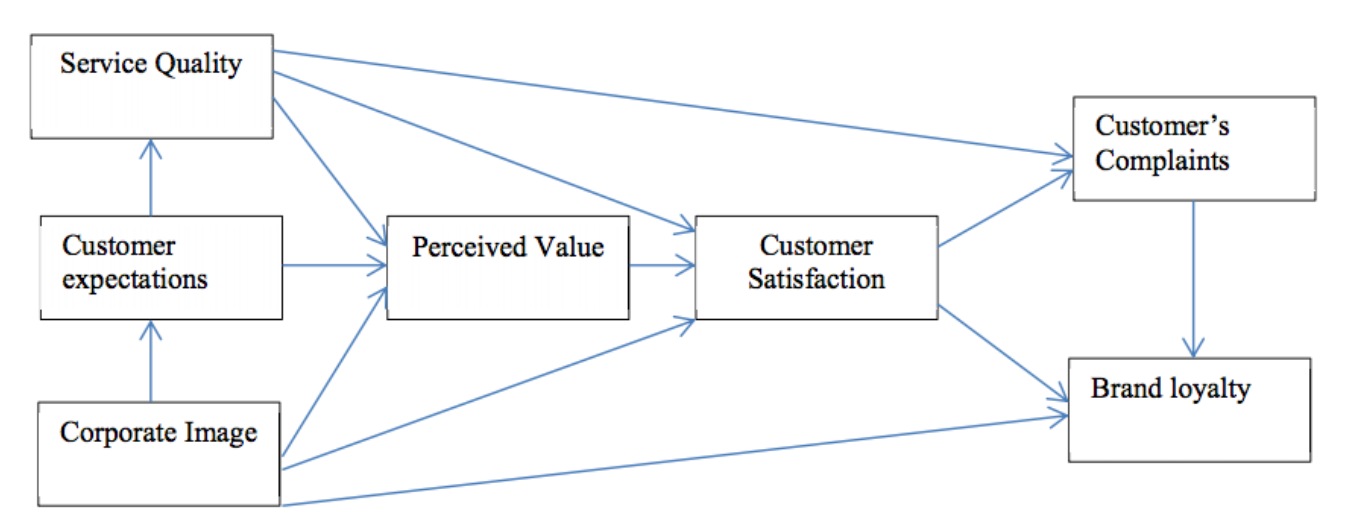
\includegraphics[width=1.0\textwidth]{img/hussain2015service.png}
	\caption{Customer satisfaction model \cite{hussain2015service}}
	\label{fig:custSatisfactionModel}
\end{figure} 

This model conforms in most parts with the opinions of \cite{neckel2015} as it indicates a strong relationship between service quality and Customer Satisfaction. The perceived value describes the subjectively perceived ratio between quality and price. If this number appears to be high for a customer, it indicates correct marketing activities. As a result the perceived value directly affects customer satisfaction as well. In addition \cite{hussain2015service} also claims that the reputation (indicated as Corporate Image in the figure) of the company influences satisfaction. Although this variable plays a role in this model it will not be considered as a core point in the practical work which puts its focus on service usage- and quality influences. What \cite{neckel2015} does not outline is the reaction of a customer itself. According to \cite{jahanshani2014study} this can be called the response of a customer which has a specific focus. This focus is hard to define in a unique way since it can have various facades. A positive experience with a product leads to an emotional effect which can for instance create happiness as temporary condition but it can also have a behavioral impact which can yield changes in the usage or attitude towards the product. Moreover according to \cite{hussain2015service} there is the statistic that a dissatisfied customer tells on average nine other people about his/her negative experiences with the product or company. With the heavy use of the Internet and social media this can get spread even faster \cite{neckel2015}. \cite{jahanshani2014study} mentions as third dimension that a customer response does not remain stable over time and varies among product usages. These changes over time are caused by several types of actions like an interaction with the product or after a purchase. This fact emphasizes that measuring customer satisfaction is an ongoing process which requires much more than an occasional estimation once in time to do it right. Although influencing factors like emotions or current mood are not accessible to the service provider at any time there is still some chance to analyze reflected information of users to gather insights into what causes a user to be more (dis)satisfied and to reason about his/her satisfaction level.

\subsection{Customer Loyalty}
\label{ssec:custLoyalty}
A customer is referred as loyal if he/she shows a positive attitude towards the service provider and thus recommends the company and its products to other people and also is willing to stay with the company in the future. Only if these two conditions are both met a customer can be clearly considered as loyal. There is also the possibility that he/she stays with the company over a longer period and does several purchases but only because there are too few other possibilities on the market ore switching to a competitor requires too much effort \cite{neckel2015}.
The customer satisfaction model of \cite{hussain2015service} indicates the loyalty parameter with "brand loyalty" and agrees with the opinion of \cite{neckel2015} with regard to a direct relationship between customer satisfaction and loyalty. Even though there is no clear evidence for causal relationship between customer satisfaction and customer loyalty so far, it has been found out that these two variables correlate positively. Customers who are satisfied with the overall product package including the provided services are more likely to buy again and stay with the company. In contrast, unsatisfied customers can cause big financial damage since they are not only vulnerable themselves to end the relationship but also influence other interested people and potential customers negatively \cite{neckel2015}. Loyal customers positively impact profitability by increasing sales due to repetitive purchases, reducing marketing and operational costs because people know certain products and do not demand for much more specific information anymore \cite{bowen2001relationship}. The difficulty is to retain a rather high number of loyal customers since small mistakes can lead to an abrupt end of the customer relationship \cite{chen2003understanding}. 

\subsection{Customer- and Company Value}
% TODO

\subsection{Customer data}
Due to the ongoing innovation in computer and software technology, businesses can collect huge amounts of data of their customers and integrate it in a way to be able to gain deep knowledge on the behavior, situations, desires and problems of them. Advanced data mining techniques allow to analyze behavior patterns of customers and predict future events and actions taken by them. The computational power of todays hardware enables businesses to store every single touch point of each customer in database systems and disregarded of the communication channel integrate it into a data warehouse to provide a comprehensive view onto the profile of a customer \cite{chen2003understanding}. Although the recent technology progress opens a wide range of new opportunities to record and monitor communication and interaction of customers with a business, it turns out that measuring satisfaction of customers and pro-actively reacting to his/her situation is a complex task \cite{neckel2015}.

\section{Thesis Statement}

\subsection{Problem}
Since the strength of customer satisfaction is connected to the attitude and loyalty towards the providing company, it turns out to be an important indicator for revenue and company value. Research showed that an 5\% increase of customer retention has a positive impact of 25 to 125\% on the profit \cite{bowen2001relationship}. Many modern Internet businesses try to live the "Customer first" principle and therefore invest resources to make their customers as satisfied as possible. They usually employ a first-class customer support service to quickly tackle problems and complaints which undoubtedly is important but since on average only 5\% of the customers actually contact customer support service when experiencing problems it demands for more sophisticated solutions to understand customers in detail \cite{neckel2015}. The big issue in reasoning about satisfaction is that it cannot be directly measured and determined whether a customer is satisfied or not. Online surveys have become quite popular to collect data about attitude and satisfactory level of customers but they lack of covering every parameter which can have some influence on how people feel about a product or service. Moreover they only reflect the current situation and therefore do not include any past events and touch points. Exactly these experiences in the past could have changed customers minds \cite{neckel2015}. To be able to explore a customer in more detail, new methods and techniques in the field of data mining have been proposed \cite{neckel2015}. 

\subsection{Research objectives}
The research question this thesis deals with is to find out how to leverage useful data related to the behavior of customers, interaction with a service respectively product and reported data from product usage, to derive patterns which allow to make a statement about how (dis)satisfied a customer is. Furthermore the results should show which data have major influence on customers satisfactory level and thus outline the essential product characteristics a service provider has to pay attention to. If the results can be considered as reliable and valid, they can be used for early detection of unsatisfied customers and help to pro-actively solve their problems. 
The route towards the goal of the research looks the following:
\begin{itemize}
	\item Define what customer satisfaction means and how to differentiate between satisfactory levels.
	\item Elaborate which data has potential to influence customer satisfaction regarding the case study example used in this research. 
	\item Find a way to represent Customer Satisfaction as reliable and measurable metric.
	\item Implement statistical tests to find out which metrics in the data affect Customer Satisfaction. 
	\item Implement a software solution to analyze behavior of customers, learn from this data and do a predictive analysis of how (dis)satisfied an arbitrary customer will be.
\end{itemize}

\section{Case Study: Tractive}
\label{sec:illustrationExample}

As representative example the research relies on the data of a pet tracking company named Tractive GmbH. The company which was founded as a startup in 2012 in Pasching, Upper Austria produces hardware devices and software applications for different kinds of pets. Their most popular product is a GPS (Global Positioning System) device which can be put on a pet and allows the customer to track its position live on a mobile phone or via a website. This way Tractive helps pet owners worldwide not to lose their pets again since they can always have a eye on them via a smartphone or desktop computer. Since the company is quite successful with about 50k paying customers using a Tractive GPS device, there is also a lot of data available related to each customer. This starts with data related to the usage of the hardware device ranging to subscription data of a customer and his/her interaction with customer support service. Since the company is built up on a subscription model which requires customers to pay on a regular basis for the usage of the device, there is special interest in binding customers for a long time to the company. In essence, this means that satisfied customers are a key asset for the company. Therefore its model should fit well to the research objectives and promising results could support solving customer issues earlier and as a result affect drop out rate positively. 

\begin{figure}[H]
	\centering
		
\includegraphics[width=0.6\textwidth]{img/tractiveLogo.jpg}%
	\caption{Tractive - Official company logo}	
\end{figure}

\section{Structure of the Thesis}

The thesis will contribute to a more efficient way of measuring customer satisfaction using large sets of collected data related to usage behavior. Chapter~\ref{ch:intro} first gave an introduction about the general problem context and outlined the research objectives as well as the illustration example this thesis is based on. Chapter~\ref{ch:backgroundResearch} will take a closer look at related research work. It will give an overview on existing approaches to determine customer satisfaction and reasons about their efficiency, problems and improvement potential. Moreover this chapter outlines necessary background research done to gain a deeper understanding on what it means to reason about satisfaction and sheds some light onto different methods suitable for the implementation part. After the fundament has been built, chapter~\ref{ch:implementation} illustrates the practical implementation in detail. Chapter~\ref{ch:evaluation} evaluates the outcome from the implementation and analyzes why some approaches work better than others. Chapter~\ref{ch:conclusion} concludes the work by summarizing the important findings and gives a short look into future work.